%! TEX TS-program = LuaLaTeX

% Gemini theme
% See: https://rev.cs.uchicago.edu/k4rtik/gemini-uccs
% A fork of https://github.com/anishathalye/gemini

\documentclass[12pt, usenames, dvipsnames]{beamer}

% ====================
% Packages
% ====================

\usepackage[T1]{fontenc}
\usepackage{lmodern}
\usepackage[size=custom, width=121.92, height=91.44, scale=1]{beamerposter}
\usetheme{gemini}
\usecolortheme{stanford}

\usepackage{graphicx}
\usepackage{booktabs}

\usepackage{hyperref}
\usepackage{amsthm}
\usepackage{thmtools}

% For theorems and such
\usepackage{amsmath}
\usepackage{amssymb}
\usepackage{mathtools}

\usepackage{natbib}

\usepackage{xcolor}
\usepackage{algorithm}
\usepackage{algorithmic}
\usepackage{bbm}
\usepackage[symbol]{footmisc}

\renewcommand{\thefootnote}{\fnsymbol{footnote}}

% ====================
% Lengths
% ====================

% If you have N columns, choose \sepwidth and \colwidth such that
% (N+1)*\sepwidth + N*\colwidth = \paperwidth
\newlength{\sepwidth}
\newlength{\colwidth}
\setlength{\sepwidth}{0.025\paperwidth}
\setlength{\colwidth}{0.30\paperwidth}

\newcommand{\separatorcolumn}{\begin{column}{\sepwidth}\end{column}}

%% load custom macros and pre-defined symbols
%% Math macros for LaTex Projects 
%% Maintainer: Aaron Mishkin <amishkin@cs.stanford.edu>
%% Original Source: Mark Schmidt (UBC CS), Ben Bloem-Reddy (UBC Stats).

%% Easy bold-face 

\def\bfA{\mathbf{A}}
\def\bfB{\mathbf{B}}
\def\bfC{\mathbf{C}}
\def\bfD{\mathbf{D}}
\def\bfE{\mathbf{E}}
\def\bfF{\mathbf{F}}
\def\bfG{\mathbf{G}}
\def\bfH{\mathbf{H}}
\def\bfI{\mathbf{I}}
\def\bfJ{\mathbf{J}}
\def\bfK{\mathbf{K}}
\def\bfL{\mathbf{L}}
\def\bfM{\mathbf{M}}
\def\bfN{\mathbf{N}}
\def\bfO{\mathbf{O}}
\def\bfP{\mathbf{P}}
\def\bfQ{\mathbf{Q}}
\def\bfR{\mathbf{R}}
\def\bfS{\mathbf{S}}
\def\bfT{\mathbf{T}}
\def\bfU{\mathbf{U}}
\def\bfV{\mathbf{V}}
\def\bfW{\mathbf{W}}
\def\bfX{\mathbf{X}}
\def\bfY{\mathbf{Y}}
\def\bfZ{\mathbf{Z}}

% bb series
\def\bbA{\mathbb{A}}
\def\bbB{\mathbb{B}}
\def\bbC{\mathbb{C}}
\def\bbD{\mathbb{D}}
\def\bbE{\mathbb{E}}
\def\bbF{\mathbb{F}}
\def\bbG{\mathbb{G}}
\def\bbH{\mathbb{H}}
\def\bbI{\mathbb{I}}
\def\bbJ{\mathbb{J}}
\def\bbK{\mathbb{K}}
\def\bbL{\mathbb{L}}
\def\bbM{\mathbb{M}}
\def\bbN{\mathbb{N}}
\def\bbO{\mathbb{O}}
\def\bbP{\mathbb{P}}
\def\bbQ{\mathbb{Q}}
\def\bbR{\mathbb{R}}
\def\bbS{\mathbb{S}}
\def\bbT{\mathbb{T}}
\def\bbU{\mathbb{U}}
\def\bbV{\mathbb{V}}
\def\bbW{\mathbb{W}}
\def\bbX{\mathbb{X}}
\def\bbY{\mathbb{Y}}
\def\bbZ{\mathbb{Z}}

% cal series
\def\calA{\mathcal{A}}
\def\calB{\mathcal{B}}
\def\calC{\mathcal{C}}
\def\calD{\mathcal{D}}
\def\calE{\mathcal{E}}
\def\calF{\mathcal{F}}
\def\calG{\mathcal{G}}
\def\calH{\mathcal{H}}
\def\calI{\mathcal{I}}
\def\calJ{\mathcal{J}}
\def\calK{\mathcal{K}}
\def\calL{\mathcal{L}}
\def\calM{\mathcal{M}}
\def\calN{\mathcal{N}}
\def\calO{\mathcal{O}}
\def\calP{\mathcal{P}}
\def\calQ{\mathcal{Q}}
\def\calR{\mathcal{R}}
\def\calS{\mathcal{S}}
\def\calT{\mathcal{T}}
\def\calU{\mathcal{U}}
\def\calV{\mathcal{V}}
\def\calW{\mathcal{W}}
\def\calX{\mathcal{X}}
\def\calY{\mathcal{Y}}
\def\calZ{\mathcal{Z}}


%% Theorem Environments %%

%% Stochastic Relations %% 

% almost sure:
\newcommand{\as}[1]{\stackrel{\text{\rm\tiny a.s.}}{#1}}
% a.s.\ equality:
\newcommand{\equas}{\stackrel{\text{\rm\tiny a.s.}}{=}}

% in distribution:
\newcommand{\dist}[1]{\stackrel{\text{\rm\tiny dist}}{#1}}
% equality in distribution:
\newcommand{\equdist}{\stackrel{\text{\rm\tiny dist}}{=}}

% independent
\newcommand{\ind}[0]{\perp \!\!\! \perp }

%% Variance, Expectation, etc %%
\newcommand{\Var}[1]{\textbf{Var}\sbr{#1}}

% ceiling and floor
\DeclarePairedDelimiter{\ceil}{\lceil}{\rceil}
\DeclarePairedDelimiter{\floor}{\lfloor}{\rfloor}
\newcommand{\argdot}{{\,\vcenter{\hbox{\tiny$\bullet$}}\,}} %generic argument dot

% absolute value
\newcommand{\abs}[1]{\left\vert #1\right\vert}

\newcommand{\seq}[1]{\rbr{#1}}

% easy bracketing:
\newcommand{\rbr}[1]{\left(#1\right)}
\newcommand{\sbr}[1]{\left[#1\right]}
\newcommand{\cbr}[1]{\left\{#1\right\}}
\newcommand{\abr}[1]{\left\langle#1\right\rangle}

% Norms
\def\norm#1{\left\|#1\right\|}
\def\biggnorm#1{\bigg\|#1\bigg\|}
% Random Variable Norms:
\def\psitwo#1{\|#1\|_{\psi_2}}
\def\psione#1{\|#1\|_{\psi_1}}

% mid
\newcommand{\biggmid}{\bigg \vert }

% argmax/argmin
\def\argmax{\mathop{\rm arg\,max}}
\def\argmin{\mathop{\rm arg\,min}}

% General Symbols
\def\half{\frac 1 2}
\newcommand{\inv}[1]{\frac{1}{#1}}
\newcommand{\halved}[1]{\frac{#1}{2}}
\newcommand{\R}{\mathbb{R}}
\newcommand{\eR}{\bar{\mathbb{R}}}

\newcommand{\into}{\rightarrow}

% Gradient Descent Symbols
\newcommand{\oracle}{\mbox{\( \calO \)}}
\newcommand{\iter}{k}

\newcommand{\Lk}{L_{\zk}}
\newcommand{\Lmax}{L_{\text{max}}}
\newcommand{\mumax}{\mu_{\text{max}}}
\newcommand{\Lmin}{L_{\text{min}}}
\newcommand{\mumin}{\mu_{\text{min}}}

% iterates
\newcommand{\y}{y}
\newcommand{\yk}{y_k}
\newcommand{\ykk}{y_{k+1}}

\newcommand{\vk}{v_k}
\newcommand{\vkk}{v_{k+1}}

\newcommand{\w}{w}
\newcommand{\wk}{w_k}
\newcommand{\wkk}{w_{k+1}}
\newcommand{\wopt}{w^*}
\newcommand{\wbar}{\bar{w}}


\newcommand{\x}{x}
\newcommand{\xk}{x_k}
\newcommand{\xkplus}{x_k^+}
\newcommand{\xkk}{x_{k+1}}
\newcommand{\xopt}{x^*}
\newcommand{\xbar}{\xbar{x}}

% noise
\newcommand{\Z}{Z}
\newcommand{\z}{z}
\newcommand{\zk}{z_{k}}
\newcommand{\zkk}{z_{k+1}}
% step-sizes
\newcommand{\tetak}{{\tilde{\eta}}_{k}}
\newcommand{\etamin}{\eta_{\text{min}}}
\newcommand{\etamax}{\eta_{\text{max}}}
\newcommand{\etak}{\eta_k}
\newcommand{\etakk}{\eta_{k+1}}

\newcommand{\betak}{\beta_{k}}
\newcommand{\betakk}{\beta_{k+1}}
\newcommand{\alphak}{\alpha_{k}}
\newcommand{\alphakk}{\alpha_{k+1}}

\newcommand{\Ek}{\bbE_{\zk}}
\newcommand{\E}{\bbE}

% functions
\newcommand{\f}{f}
\newcommand{\fj}{f_i}
\newcommand{\fopt}{f^*}
% sub-sampled functions
\newcommand{\fk}{f_{i_k}}
\newcommand{\fkk}{f_{i_{(k+1)}}}
% gradients
\newcommand{\grad}{\nabla f}
% sub-sampled gradients
\newcommand{\gradk}{\nabla f_{i_k}}
\newcommand{\gradkk}{\nabla f_{i_{(k+1)}}}

%% Weak and strong growth constants
\newcommand{\sgc}{\rho}
\newcommand{\wgc}{\alpha}

%% matrix operators
\newcommand{\diag}{\text{diag}}


%%%%%%%%%%%%%%%%%%%%%%%%%%%%%%%%%%%%%%%%%%%%%%%%%%%%%%%%%%

%% Etc %%  

%% add numbers to align* environments.
\newcommand{\addnumber}{\addtocounter{equation}{1}\tag{\theequation}}

%%%%%%%%%

%% macros for paragraph mode
%% Paragraph-Mode Macros for Latex Projects 
%% Maintainer: Aaron Mishkin <amishkin@cs.stanford.edu>


%% Text Colors %%

\newcommand{\aside}[1]{(\textcolor{red}{\textbf{Aside}: #1})}


%% tikz

\usepackage{tikz}
\usepackage{pgfplots}
\pgfplotsset{
	compat=1.16,
	oracle/.style={color=bad, style=solid, line width=1.5pt},
	bound/.style={color=blue, style=solid, line width=1.5pt},
	objective/.style={color=black, style=solid, line width=1.5pt},
}
%% Plotting macros for LaTex Projects 
%% Maintainer: Aaron Mishkin <amishkin@cs.stanford.edu>


%% Tikz and PGFplots packages
\usepackage{tikz}
\usepackage{pgfplots}

% tikz and PGFplots libraries
\usepgfplotslibrary{fillbetween}
\usetikzlibrary{patterns}



%% tikz settings 
\tikzset{
    font={\fontsize{12pt}{12}\selectfont},
}

%% PGFplots settings 
\pgfplotsset{
    % version compatibility
    compat=1.5.1,
    % basic line-styles
    primary/.style={color=black, style=solid, line width=1.5pt}, 
    secondary/.style={color=red, style=solid, line width=1.5pt}, 
}

\usetikzlibrary{shapes, arrows}
\usetikzlibrary{decorations.pathreplacing, calligraphy, calc}
\usepgfplotslibrary{fillbetween}

\definecolor{BurntOrange}{HTML}{CC5500}
\definecolor{DarkFern}{HTML}{407428}
\definecolor{CBRed}{HTML}{994F00}
\definecolor{CBBlue}{HTML}{006CD1}
\colorlet{Fern}{DarkFern!85!white}
\colorlet{LightFern}{DarkFern!20!white}

\colorlet{LightCerulean}{CBBlue!20!white}
\setbeamercolor{result}{bg=LightCerulean}
\setbeamercolor{headline}{bg=white,fg=cardinalred}

\definecolor{bad}{HTML}{eb6223}
\definecolor{good}{HTML}{9434ed}
\newcommand{\bad}[1]{\textcolor{bad}{#1}}
\newcommand{\good}[1]{\textcolor{CBBlue}{#1}}

\newcommand{\red}[1]{\textcolor{Red}{#1}}
\newcommand{\green}[1]{\textcolor{ForestGreen}{#1}}
\newcommand{\blue}[1]{\textcolor{CBBlue}{#1}}
\newcommand{\purple}[1]{\textcolor{Magenta}{#1}}

\newcommand{\horizontalrule}{
	{
			\vspace{-0.5em}
            \begin{center}
			\rule{0.6\textwidth}{0.1em}
            \end{center}
			\vspace{-0.2em}
		}
}


\title{Directional Smoothness and Gradient Methods: Convergence and Adaptivity}

\author{Aaron Mishkin* \inst{1}%
	\and Ahmed Khaled* \inst{2}% 
    \and Yuanhao Wang \inst{2}%
	\and Aaron Defazio \inst{3}% 
	\and Robert M. Gower \inst{4}}

\institute[shortinst]{\inst{1} Stanford University \samelineand \inst{2} Princeton University \samelineand \inst{3} FAIR, META \samelineand \inst{4} CCM, Flatiron Institute}

% ====================
% Footer (optional)
% ====================

\footercontent{
	\textbf{NeurIPS 2024} \hfill \textbf{$^*$ Equal Contribution}\hfill
	\textbf{Correspondence}: \href{mailto:amishkin@cs.stanford.edu}{amishkin@cs.stanford.edu}}
% (can be left out to remove footer)

% ====================
% Body
% ====================

\begin{document}

% This adds the Logos on the top left and top right
\addtobeamertemplate{headline}{}
{%
    \begin{tikzpicture}[remember picture,overlay]
        \node [anchor=north west, inner sep=3cm] at ([xshift=0.0cm,yshift=-3.0cm]current page.north west)
        {
\includegraphics[height=2.5cm]{assets/institutes/ccm.png}};
        \node [anchor=north west, inner sep=3cm] at ([xshift=0.5cm,yshift=2.0cm]current page.north west)
        {
\includegraphics[height=5.5cm]{assets/institutes/meta_logo.png}};
        \node [anchor=north east, inner sep=3cm] at ([xshift=-1.0cm,yshift=1.85cm]current page.north east)
        {
\includegraphics[height=5.0cm]{assets/institutes/stanford.png}};
        \node [anchor=north east, inner sep=3cm] at ([xshift=0.0cm,yshift=-2.00cm]current page.north east)
        {
\includegraphics[height=5.0cm]{assets/institutes/princeton.png}};
    \end{tikzpicture}
}%

\begin{frame}[t]
    \large
    \vspace{-2.5ex}
    \begin{columns}[t]
        \separatorcolumn
        \begin{column}{\colwidth}
            \begin{block}{Introduction}
                {\Large
                    \textbf{Goal}: Minimize convex, differentiable function \( f \) using
                    GD,
                    \[
                        \xkk = \xk - \etak \grad(\xk).
                    \]
                }
                %\vspace{-1ex}

                {\Large
                    \textbf{Problem}: Gradient descent (GD) is an inherently \good{local algorithm},
                    but standard analyses rely on \bad{global, worst-case} assumptions.%
                }
                \vspace{-1.5ex}
                \begin{columns}[t]
                    \begin{column}{0.5\textwidth}
                        \begin{center}
                            \Large \textbf{\bad{Global Smoothness}}
                        \end{center}
                        \vspace{-2ex}

                        \begin{figure}[]
                            \centering
                            %! TEX root = ../../main.tex
%% Illustration of step-sizes bound from Armijo line-search. 

\begin{tikzpicture}[
        declare function={
                objective(\x)=      (\x<=0) * (pow(\x, 2)*0.8 - 1*\x)
                + (\x>0) * (2.0*pow(\x, 3) - 2 * \x^2 - 1*\x);
                objectivePrime(\x)=      (\x<=0) * (2*\x*0.8 - 1)
                + (\x>0) * (6.0*pow(\x, 2) - 4 * \x - 1);
                upperBound(\x)=     ( 2.5*pow(\x, 2) - 1*\x);
                M(\x) = 1.2*abs(objectivePrime(\x) + 1) / abs(\x);
                directionalSmoothness(\x) = -1 * \x
                + M(\x) * pow(\x, 2) / 2;
            }
    ]
    \begin{axis}[
            width=0.5\textwidth,
            height=6cm,
            axis x line=none, axis y line=none,
            ymin=-1.5, ymax=7, ytick={-5,...,7}, ylabel=$y$,
            xmin=-2.5, xmax=5, xtick={-5,...,5}, xlabel=$x$,
            restrict y to domain=-3.25:10,
            scale=3.5,
        ]

        \addplot[name path=function, domain=-3.5:5.5, samples=200, objective, line width=8pt]{objective(x)};
        %\addplot[name path=directionalSmoothness, domain=-3.5:5.5, samples=300, bound, line width=8pt]{directionalSmoothness(x)};
        \addplot[name path=upperBound, domain=-3.5:5.5, samples=200, oracle, line width=8pt]{upperBound(x)};

        \node[label={[font=\huge]270:$\xk$},circle,fill,inner sep=6pt] at (axis cs:0,0) {};

        \node[label={[font=\huge]180:$f(w)$}] at (axis cs:3,1) {};
        \node[label={[font=\Large]0:$L$-Smooth}] at (axis cs:-1.4,6) {};
        \node[label={[font=\Large]0:Bound}] at (axis cs:-1.1,5.2) {};
        %\node[label={0:{$\ell_{v_k}(\eta)$}}] at (axis cs:3.6,-2.4) {};
        %\node[label={180:{$h_{v_k}(\eta)$}}] at (axis cs:0.3,3) {};

        \addplot fill between[
                of = function and upperBound,
                %split, % calculate segments
                every even segment/.style = {fill=red, fill opacity=0.3},
                every odd segment/.style  = {fill=red, fill opacity=0.3}
            ];

    \end{axis}

\end{tikzpicture}

                        \end{figure}
                    \end{column}
                    \begin{column}{0.5\textwidth}
                        \begin{center}
                            \Large \textbf{\good{Directional Smoothness}}
                        \end{center}
                        \vspace{-2ex}

                        \begin{figure}[]
                            \centering
                            %! TEX root = ../../main.tex
%% Illustration of step-sizes bound from Armijo line-search. 

\begin{tikzpicture}[
        declare function={
                objective(\x)=      (\x<=0) * (pow(\x, 2)*0.8 - 1*\x)
                + (\x>0) * (2.0*pow(\x, 3) - 2 * \x^2 - 1*\x);
                objectivePrime(\x)=      (\x<=0) * (2*\x*0.8 - 1)
                + (\x>0) * (6.0*pow(\x, 2) - 4 * \x - 1);
                upperBound(\x)=     ( 1.75*pow(\x, 2) - 1*\x);
                M(\x) = 1.2*abs(objectivePrime(\x) + 1) / abs(\x);
                directionalSmoothness(\x) = -1 * \x
                + M(\x) * pow(\x, 2) / 2;
            }
    ]
    \begin{axis}[
            width=0.5\textwidth,
            height=6cm,
            axis x line=none, axis y line=none,
            ymin=-1.5, ymax=7, ytick={-5,...,7}, ylabel=$y$,
            xmin=-2.5, xmax=5, xtick={-5,...,5}, xlabel=$x$,
            restrict y to domain=-3.25:10,
            scale=3.5,
        ]

        \addplot[name path=function, domain=-3.5:5.5, samples=200, objective, line width=8pt]{objective(x)};
        \addplot[name path=directionalSmoothness, domain=-3.5:5.5, samples=300, bound, line width=8pt]{directionalSmoothness(x)};
        %\addplot[name path=upperBound, domain=-3.5:5.5, samples=200, oracle, line width=8pt]{upperBound(x)};

        \node[label={[font=\huge]270:$\xk$},circle,fill,inner sep=6pt] at (axis cs:0,0) {};

        \node[label={[font=\huge]180:$f(w)$}] at (axis cs:3,1) {};
        \node[label={[font=\Large]180:$M(\xk, y)$-Smooth}] at (axis cs:1,6) {};
        \node[label={[font=\Large]180:Bound}] at (axis cs:0.1,5.2) {};
        %\node[label={0:{$\ell_{v_k}(\eta)$}}] at (axis cs:3.6,-2.4) {};
        %\node[label={180:{$h_{v_k}(\eta)$}}] at (axis cs:0.3,3) {};

        \addplot fill between[
                of = function and directionalSmoothness,
                split, % calculate segments
                every odd segment/.style = {fill=green, fill opacity=0.3},
                every even segment/.style  = {fill=green, fill opacity=0.3}
            ];

    \end{axis}

\end{tikzpicture}

                        \end{figure}
                    \end{column}
                \end{columns}
                {\Large \textbf{Main Contributions}:}
                \vspace{-1.5ex}
                \begin{itemize}
                    \item \good{Directional Smoothness}:
                          a new, point-wise relaxation of \( L \)-smoothness.

                    \item \good{Path-Dependent Rates}:
                          guarantees for GD using only local properties of \( f \).

                    \item \good{Adaptive Methods}:
                          optimizers that adapt to the directional smoothness.
                \end{itemize}
            \end{block}
            \vspace{-1.5ex}
            \begin{block}{Directional Smoothness}

                {\Large%
                    \textbf{Global Smoothness}: \( f \) is \bad{\( L \)-smooth} if for every
                    \( x, y \in \text{dom}(f)\),
                    \[
                        f(y) \leq f(x) + \abr{\grad(x), y - x} + \frac{\bad{L}}{2}\norm{y - x}_2^2,
                    \]
                }%

                {\Large%
                    \textbf{Directional Smoothness}: \( M \) is a
                    \good{directional smoothness function} if,
                    \[
                        f(y) \leq f(x) + \abr{\grad(x), y - x} + \frac{\good{M(x, y)}}{2}\norm{y - x}_2^2.
                    \]
                }%

                {\Large
                    We give \good{explicit} smoothness functions --- no oracles required!
                }

                \horizontalrule

                {\Large
                    \textbf{Point-wise Smoothness}:
                    \vspace{2ex}
                    \[
                        D(x, y) =
                        \frac{\bad{2} \norm{\grad(x) - \grad(y)}_2}{\norm{x - y}_2}
                        \hspace{19.4ex}
                        (\bad{\leq 2L})
                    \]

                    \textbf{Path-wise Smoothness}:
                    \vspace{2ex}
                    \[
                        A(x, y) =
                        \bad{\sup_{t \in [0, 1]}}
                        \frac{\abr{\grad(x + \bad{t}(y - x)) - \grad(x), y - x}}
                        {\bad{t}\norm{x - y}_2^2}
                        \hspace{3ex}
                        (\good{\leq L})
                    \]

                    \textbf{Exact (Point-wise) Smoothness}:
                    \vspace{2ex}
                    \[
                        H(x, y) =
                        \frac{2\abs{f(y) - f(x) - \abr{\grad(x), y - x}}}{\norm{y - x}_2^2}
                        \hspace{8.7ex}
                        (\good{\leq L})
                    \]
                }
                %\vspace{1ex}

                {\Large
                    Easy to \good{compute in hindsight} unlike other approaches
                    \citep{park2021preconditioned,
                        mei21_lever_non_unifor_first_order}.
                }

            \end{block}
        \end{column}

        \separatorcolumn

        \begin{column}{\colwidth}
            \begin{block}{Path-Dependent Rates}

                \begin{figure}[]
                    \centering
                    %! TEX root = ../main.tex

\begin{tikzpicture}[
      scale=2.75,
      declare function={
        objective(\x)=  (\x<=0) * pow(-\x, 3) / 2 + (\x>0) * pow(x, 2);
        upperBound(\x)=     7 * pow(\x + 1.95, 2) - 6 * (\x + 1.95) + 3.8; 
        locaUpperBound(\x)=     5 * pow(\x + 1.9, 2) - 6 * (\x + 1.9) + 3.5; 
      }
    ]
    \begin{axis}[
      width=0.4\textwidth,
      height=6cm,
      axis x line=none, axis y line=none,
      ymin=-0.5, ymax=6, ytick={-5,...,5}, ylabel=$y$,
      xmin=-3.0, xmax=1.5, xtick={-4,...,2}, xlabel=$x$,
    ]

    \addplot[name path=function, domain=-3.5:5.23, samples=300, objective, line width=2pt]{objective(x)};
    \addplot[name path=upperBound, domain=-3.5:7, samples=300, oracle, line width=2pt]{upperBound(x)};
    \addplot[name path=localUpperBound, domain=-3.5:7, samples=300, bound, line width=2pt]{locaUpperBound(x)};

    \node[label={[label distance=-0.5cm, font=\scriptsize] 195:$\xk$},circle,fill,inner sep=2pt] at (axis cs:-1.9, 3.5) {};
    \node[label={[label distance=-0.5cm, font=\scriptsize]195:$\xkk$},circle,fill,inner sep=2pt] at (axis cs:-1.5, 1.6875) {};
    \node[label={[font=\scriptsize]90:$\xopt$},circle,fill,inner sep=2pt] at (axis cs:0,0) {};
    
    \node[label={[font=\scriptsize]180:$f(x)$}] at (axis cs:1.4,0.3) {};

    \draw [line width=2pt, style=dashed, color=black] (axis cs:-2.2,1.675) -- (axis cs:-1.5, 1.675);
    \draw [line width=2pt, style=dashed] (axis cs:-2.2,3.5) -- (axis cs:-1.9, 3.5);
    \draw [decorate, decoration={brace, amplitude=4pt}, line width=2pt] (axis cs:-2.195,1.675) -- (axis cs:-2.195,3.5) node [midway, anchor=east, xshift=-1mm, outer sep=1pt,font=\tiny, align=left]{Actual\\ Progress};


    \draw [line width=2pt, style=dashed, color=black] (axis cs:-0.495,2.5) -- (axis cs:-1.41, 2.5);
    \draw [line width=2pt, style=dashed] (axis cs:-1.1,3.5) -- (axis cs:-0.495, 3.5);
    \draw [decorate, decoration={brace, amplitude=4pt, mirror}, line width=2pt] (axis cs:-0.5, 2.5) -- (axis cs:-0.5,3.5) node [midway, anchor=west, xshift=1mm, outer sep=1pt,font=\tiny]{\( L \)-Smooth};


    \draw [line width=2pt, style=dashed, color=purple] (axis cs:0.5,1.9) -- (axis cs:-1.06, 1.9);
    \draw [line width=2pt, style=dashed, color=purple] (axis cs:-0.40,3.5) -- (axis cs:0.5, 3.5);
    \draw [decorate, decoration={brace, amplitude=4pt, mirror}, line width=2pt] (axis cs:0.497, 1.9) -- (axis cs:0.497, 3.5) node [midway, anchor=west, xshift=1mm, outer sep=1pt,font=\tiny]{\( M_k \)-Smooth};
    \end{axis}
\end{tikzpicture} 
%
                \end{figure}
                \vspace{-1.5ex}

                \begin{itemize}
                    \Large
                    \item  \good{Directional smoothness} \( \implies \)
                          more progress than \bad{\( L \)-smoothness}!
                \end{itemize}
                \vspace{-1.5ex}
                \horizontalrule

                {\Large
                    \textbf{Approach}: study \good{local behavior} of GD along
                    \( \cbr{\xk} \) using \( M(\xk, \xkk) \).
                }

                \vspace{1ex}

                \begin{beamercolorbox}[wd=\textwidth,sep=1em]{result}
                    \textbf{Proposition} (Strongly Convex):
                    Let \( \Delta_i = \norm{\x_i - \x_0}_2^2 \)
                    and \( M_i = M(\x_i, \x_{i+1}) \).
                    If \( f \) is \( \mu \)-strongly convex, then GD with
                    step-size sequence \( \cbr{\etak} \) satisfies,
                    {\Large
                            \[
                                \Delta_{k}
                                \leq \sbr{\prod_{i=0}^{k}
                                    \frac{\abs{1 \!-\! \mu \eta_i}}{1 + \mu \eta_i}} \Delta_0
                                + \sum_{i=0}^k \sbr{\prod_{j > i}
                                    \frac{\abs{1 \!-\! \mu \eta_j}}{1 + \mu \eta_j}}
                                \eta_i^2 \bad{\rbr{M_i \eta_i - 1}} \norm{\grad(\xk)}_2^2.
                            \]
                        }
                \end{beamercolorbox}
                \vspace{-1.0ex}

                {\Large
                    \begin{itemize}
                        \item \good{Fast rates} when \( \etak \) are adapted,
                              meaning \( \etak \leq 1 / M(\xk, \xkk)\).

                        \item Describes worst-case \bad{``blow-up''} when \( \etak \) are not adapted.
                    \end{itemize}
                }

                \vspace{1ex}

                \begin{beamercolorbox}[wd=\textwidth,sep=1em]{result}
                    \textbf{Proposition} (Convex):
                    Let \( \Delta_i = \norm{\x_i - \x_0}_2^2 \)
                    and \( M_i = M(\x_i, \x_{i+1}) \).
                    If \( f \) is convex, then
                    GD with step-size sequence \( \cbr{\etak} \)
                    satisfies,
                    {\Large
                            \[
                                \min_{i \in [k]} f(x_i) - f(\xopt)
                                \leq \frac{\Delta_0
                                    + \sum_{i=0}^{k} \eta_i^2 \bad{(\eta_i M_i - 1)}
                                    \norm{\grad(\x_i)}_2^2}{2\sum_{i=0}^k \eta_i},
                            \]
                        }
                \end{beamercolorbox}
                \vspace{0.5ex}

                {\Large
                    \textbf{Definition}: \( \etak \) is
                    \good{strongly adapted} to smoothness function \( M \) if,
                    \[
                        \etak = \frac{1}{M(\xk, \xk - \etak \grad(\xk))}.
                    \]
                    %\vspace{2ex}
                    %This is the directional smoothness version of
                    %``optimal'' \bad{\( \etak = 1 / L \)}!

                    \vspace{0.5ex}
                    Strongly adapted step-sizes get \good{path-dependent rates}.
                    \vspace{-1.0ex}

                    \begin{columns}[t]
                        \begin{column}{0.45\textwidth}
                            \begin{center}
                                \Large \textbf{\bad{Global Smoothness}}
                            \end{center}
                            \vspace{1ex}
                            \[
                                \min_{i \in [k]} f(x_i) - f(\xopt)
                                \leq \frac{\bad{L} \Delta_0}{k+1}
                            \]
                        \end{column}
                        \begin{column}{0.55\textwidth}
                            \begin{center}
                                \Large \textbf{\good{Directional Smoothness}}
                            \end{center}
                            \vspace{1ex}
                            \[
                                \min_{i \in [k]} f(x_i) - f(\xopt)
                                \leq \good{\sbr{\frac{\sum_{i=0}^k M_i}{k+1}}}
                                \frac{\Delta_0}{k+1}
                            \]
                        \end{column}
                    \end{columns}
                }
            \end{block}
            \begin{block}{The Quadratic Case}
                {\Large
                    \textbf{Problem}: strongly adapted \( \etak \)
                    require solving an \bad{implicit equation}.
                }
                \vspace{1ex}

                \begin{beamercolorbox}[wd=\textwidth,sep=1em]{result}
                    \textbf{Lemma}: If \( f(x) = \half x^\top B x - c^\top x \),
                    then the point-wise smoothness is given by,
                    {\Large
                            \[
                                D(\xk, \xkk(\etak))
                                = \frac{\norm{B \grad(\xk)}_2}{\norm{\grad(\xk)}_2}.
                            \]
                        }
                \end{beamercolorbox}
                \vspace{-1.0ex}
                \begin{itemize}
                    \Large
                    \item This recovers a \good{classic step-size} for quadratic
                          optimization proposed by \citet{dai2006computational}!
                \end{itemize}
            \end{block}
        \end{column}

        \separatorcolumn

        \begin{column}{\colwidth}

            \begin{block}{Adaptive Methods}
                \vspace{-.25ex}
                \begin{center}
                    {\Large
                        \textbf{Question}: Can we obtain \good{path-dependent
                        rates} for convex functions without computing
                        \bad{strongly adapted step-sizes}?
                    }
                \end{center}
                \vspace{-1.5ex}

                \horizontalrule

                {\Large
                    \textbf{First Attempt}: Modify exponential search \citep{yair2022parameter}.
                }
                \vspace{0.25ex}

                \begin{beamercolorbox}[wd=\textwidth,sep=1em]{result}
                    \textbf{Theorem} (informal): If \( f \) is convex and
                    \( L \)-smooth, then exponential search requires at most
                    \( 2 K \log \log (2 \eta_0 / L) \) iterations of GD to find
                    \( \eta^* \) yielding the path-dependent convergence rate:
                    {\Large
                    \[
                        f(\bar{x}_K) - f(\xopt)
                        \leq \frac{\norm{x_0 - x_{*}}^2}{2 K}
                        \left[ \frac{\sum_{i=0}^K M(\bad{x_{i+1}'}, \bad{x_i'})
                                \norm{\nabla f(\bad{x_i'})}^2}{\sum_{i=0}^K \norm{\nabla f(\bad{x_i'})}^2} \right],
                    \]
                    }
                \end{beamercolorbox}

                {\Large
                \textbf{Problem}: Only adapts to smoothness along \bad{virtual sequence}
                \( \cbr{\xk'} \).
                }
                \vspace{-2.5ex}
                \horizontalrule
                {\Large
                    \textbf{Second Attempt}: \good{Polyak step-size}:
                    \(
                    \etak = \gamma (f(\xk) - f(\xopt))/\norm{\grad(\xk)}_2^2
                    \)
                }

                \vspace{1ex}

                \begin{beamercolorbox}[wd=\textwidth,sep=1em]{result}
                    \textbf{Theorem} (Polyak Step-Size): If \( f \) is convex and
                    differentiable, then GD with the Polyak step-size using
                    \( \gamma = 1.5 \) satisfies,
                    {\Large
                            \[
                                \min_{i \in [k]} f(x_i) - f(\xopt)
                                \leq \bad{3} \good{\sbr{\frac{\sum_{i=0}^k M_i}{k+1}}}
                                \frac{\Delta_0}{k+1}
                            \]
                        }
                \end{beamercolorbox}
                \vspace{-1ex}
                {\Large
                    \begin{itemize}
                        \item \good{Matches rate} for strongly adapted step-sizes up to a constant!
                        \item Polyak step-size is ``adaptive'' to \good{any choice} of smoothness
                              \( M \).
                    \end{itemize}
                }

            \end{block}
            \vspace{-3ex}
            \begin{block}{Experiments}

                \begin{figure}[]
                    \centering
                    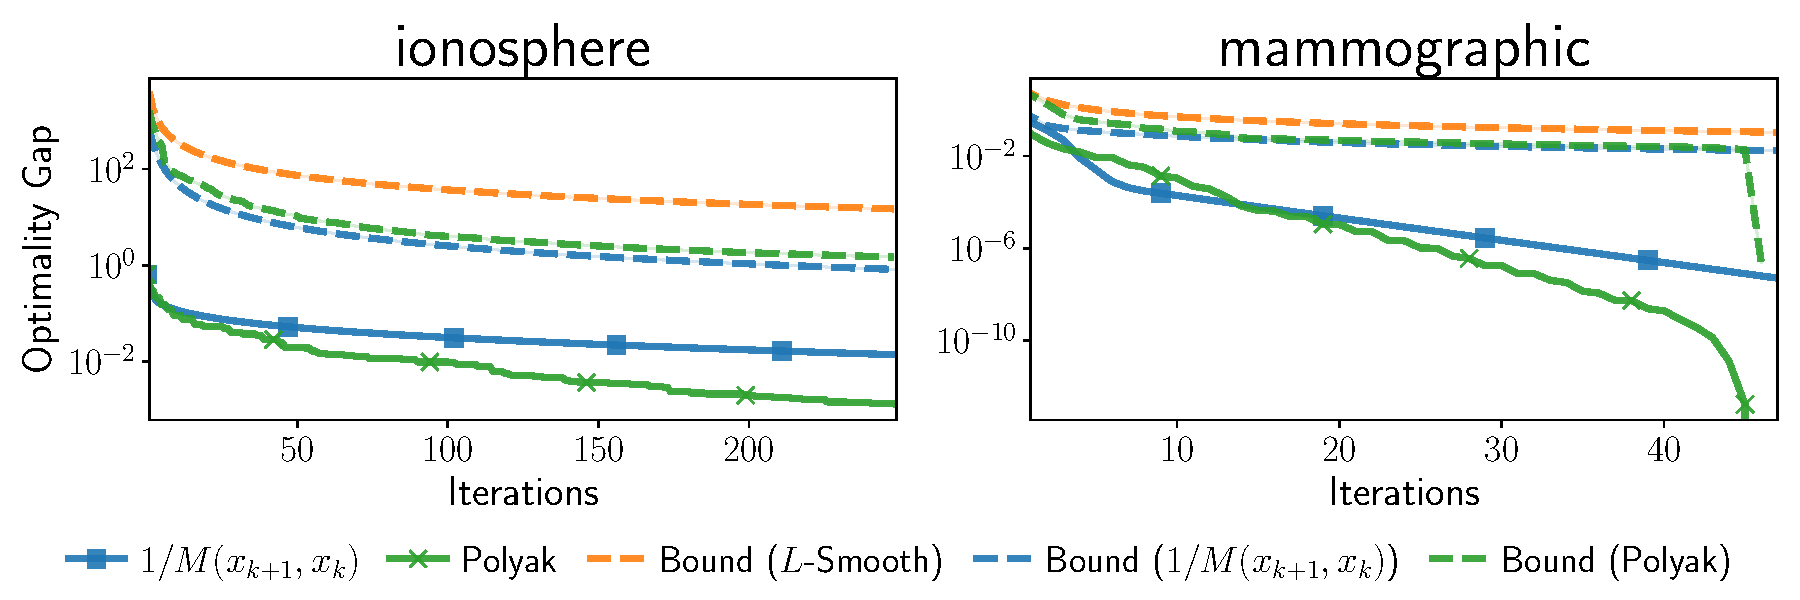
\includegraphics[width=1\textwidth]{assets/theoretical_rates.pdf}
                \end{figure}
                \vspace{-3ex}

                \begin{figure}[]
                    \centering
                    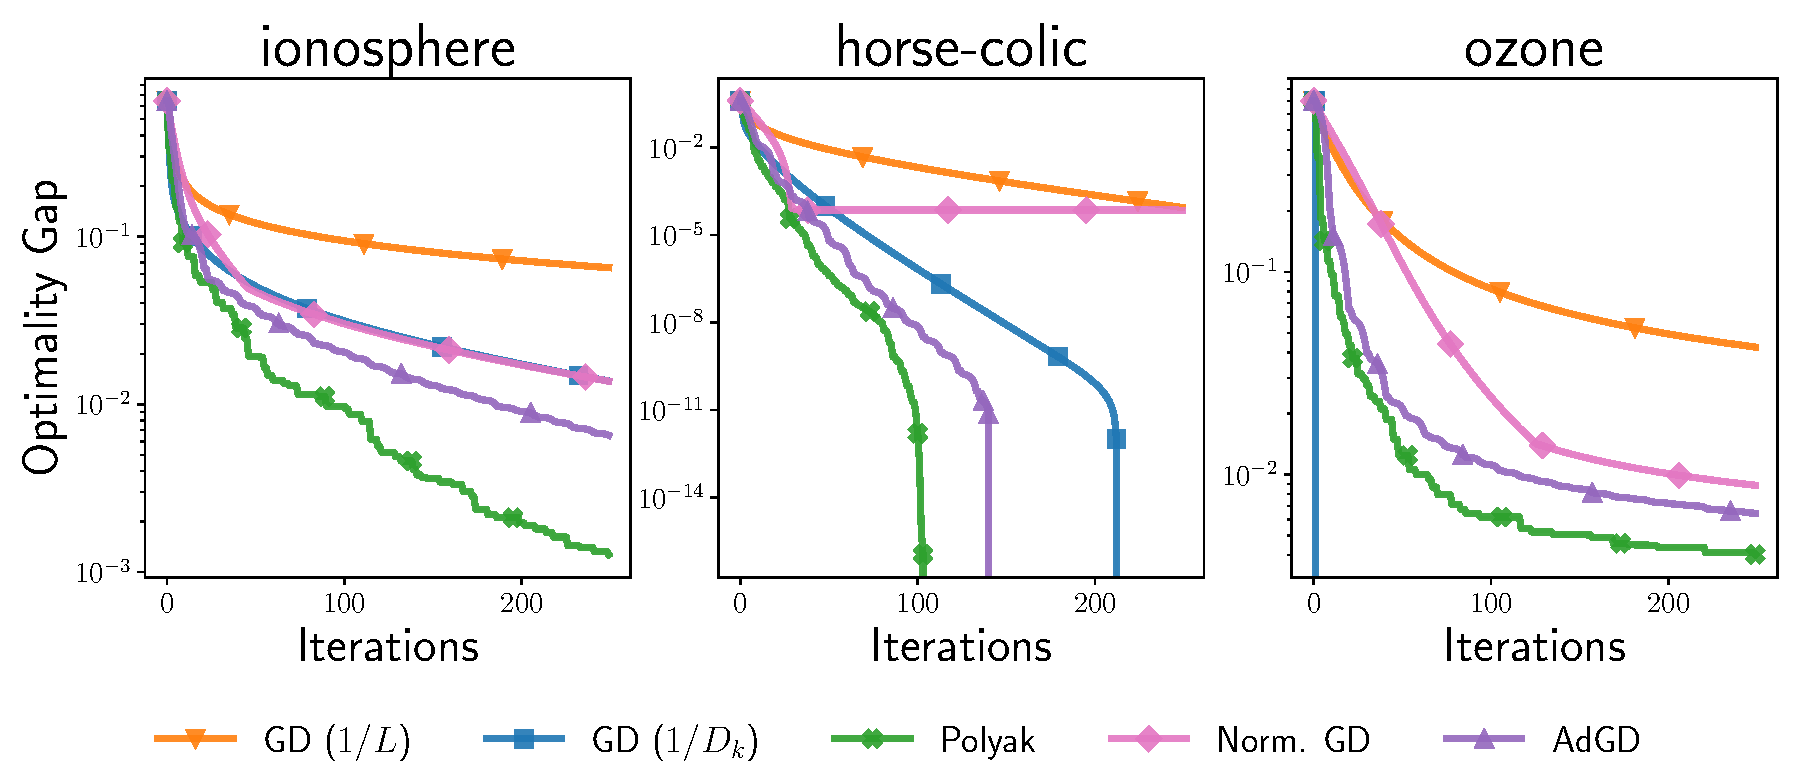
\includegraphics[width=1\textwidth]{assets/logistic_comparison.pdf}
                \end{figure}

                \vspace{-1ex}
                \underline{\textbf{References}}
                \footnotesize{
                    \bibliography{
                        refs.bib
                    }
                }
                \bibliographystyle{icml2022}

            \end{block}

        \end{column}

        \separatorcolumn
    \end{columns}
\end{frame}

\end{document}
